\begin{figure}[htb!]
    \centering
    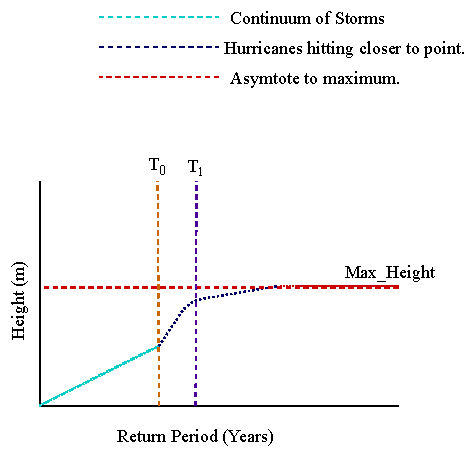
\includegraphics[width=1\linewidth]{images/Return_Hypothesis.pdf}
    \vspace{-15pt}
   \caption{The maximum height is a function of the potential intensity
   allowed by the climate, and the responsiveness of that point on the coastline to a
   wind stress of that size. If T$_0$, or T$_1$, is a similar or greater than the time period of
   measurement, then it is respectively possible that no hurricanes exist in the data sample,
   or that no hurricanes make direct landfall at that location.}
     \label{fig:return_hyp_new}

\end{figure}
